% !TeX root = 00_Vorlage.tex
% !TeX spellcheck = de_DE

\section{Aufbau und Methoden}
\label{sec:aufbau}

In diesem Kapitel wird der Aufbau der drei Einzelversuchen erläutert

\subsection{Stärke und Inklinationswinkel des Erdmagnetfelds}
\label{sec:Erdmagnetfeld}
Um systematische Fehler in den Messdaten zu vermeiden, muss als erstes sichergestellt werden, dass sich im Umkreis von circa \( 1 \unit{m} \) des Tisches keine metallischen Objekte befinden, da diese das Magnetfeld der Erde verzehren können. Danach lässt sich der Hall-Effekt Sensor im IOLab über die Software kalibrieren.
Um die Berechnung des Inklinationswinkel zu vereinfachen, muss das IOLab am Tisch so ausgerichtet werden, dass eine Komponente des gemessenen Magnetfeldes im Rahmen der Unsicherheit mit \( 0 \) vereinbar ist. Ist der Hall-Effekt Sensor so ausgerichtet, dass eine kartesische Komponente 0 ist (und somit die beiden Anderen im Betrag maximal sind) kann man die eigentliche Ausmessung vom Inklinationswinkel und Betrag des Erdmagnetfeldes durchführen.

\subsection{Elektromotor zur Bestimmung von Nord und Südpol eines Permanentmagneten} 
Für diesen Versuch werden eine AA Batterie, eine Spax-Schraube, ein Permanentmagnet und ein Kabel benötigt. Auf den Permanentmagneten wird die (am besten ferromagnetische und auf jeden Fall Stromleitende) Schraube gestellt, dessen Spitze als Drehachse fungiert. Auf die Schraubenspitze balancieren wir eine Batterie, mit dem Minuspol nach unten. Das andere Ende der Batterie verbinden wir mit einem Kabel mit dem Magneten. Hierbei ist wichtig, das Kabel am äußeren Rand des Magneten anzuschließen, da es sonst zu keiner Rotation der Batterie kommt.

Je nach Ausrichtung des Magneten geht das Magnetfeld in die positive oder negative z-Richtung und je nach Ausrichtung der Batterie fließt der Strom von der Batterie über das Kabel in den Magneten oder umgekehrt (das Koordinatensystem wurde so gelegt, dass der Strom in der xz-Ebene fließt). Wir haben also vier verschiedene Konfigurationsmöglichkeiten mit zwei unterschiedliche Beobachtungen, eine Drehung in und gegen den Uhrzeigersinn. In \autoref{fig:Motor} ist der Versuchsaufbau (links), sowie die möglichen Konfigurationsarten (rechts) dargestellt.

	\begin{figure}[H]
		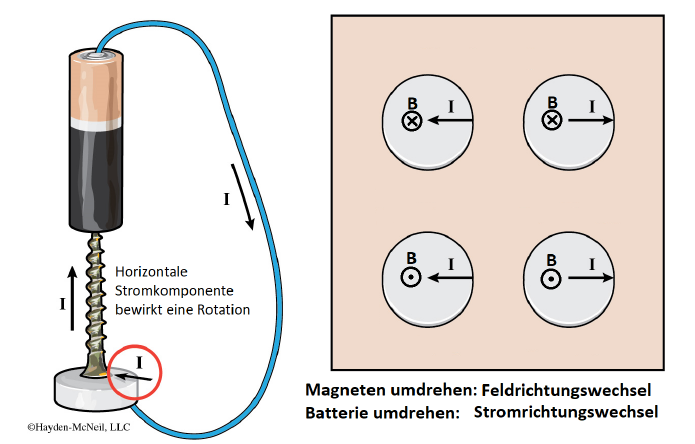
\includegraphics[width=.7\textwidth, right]{Motor}
		\caption[]{Links: Versuchsaufbau des Batteriemotors. Auf einen Permanentmagneten wird über eine Schraube eine Batterie gestellt, welche über ein Kabel wieder mit dem Magneten in der Basis verbunden ist. Rechts: möglichen Konfigurationsarten des Versuchs mit eingezeichnetem Strom und Magnetfeld. Graphik entnommen aus \footnotemark[2] }
		\label{fig:Motor}
	\end{figure}
	
	\begin{minipage}{\textwidth}
		\vspace{-13cm}
		\begin{tikzpicture}[scale=3]
			\draw[-Stealth] (0,0) -- (0,1) node [above] {\large \( z \)};
			\draw[-Stealth] (0,0) -- (1,0) node [right] {\large \( x \)};
			\draw[-Stealth] (0,0) -- (0.6,0.4) node [right] {\large \( y \)};
			
			
			\node [xshift=0.5cm] at (3.2,1.8) {\large \( 1 \)};
			\node [xshift=0.5cm] at (4,1.8) {\large \( 2 \)};
			\node [xshift=0.5cm] at (3.2,0.9) {\large \( 3 \)};
			\node [xshift=0.5cm] at (4,0.9) {\large \( 4 \)};
		\end{tikzpicture}
	\end{minipage}

\subsection{Strom durch einen langen geraden Leiter}
In diesem Versuch wird das Magnetfeld eines langen geraden Leiters gemessen, um auf den Kurschlussstrom zurückzuschließen. Dazu wird eine frische AA Batterie, ein Kabel und ein Stück Papier benötigt. Zuerst wird unter Spannung ein ungefähr \( 15 \unit{cm} \) langes Stück des Kabels mit Klebeband am Tisch befestigt. Daraufhin wird auf einem Papier eine Skala mit elf Markierungen mit jeweils $1 \unit{cm}$ Abstand gezeichnet und unter den Leiter geschoben. Der erste Strich sollte unter dem Kabel sein.
\begin{figure}[H]
	\centering
	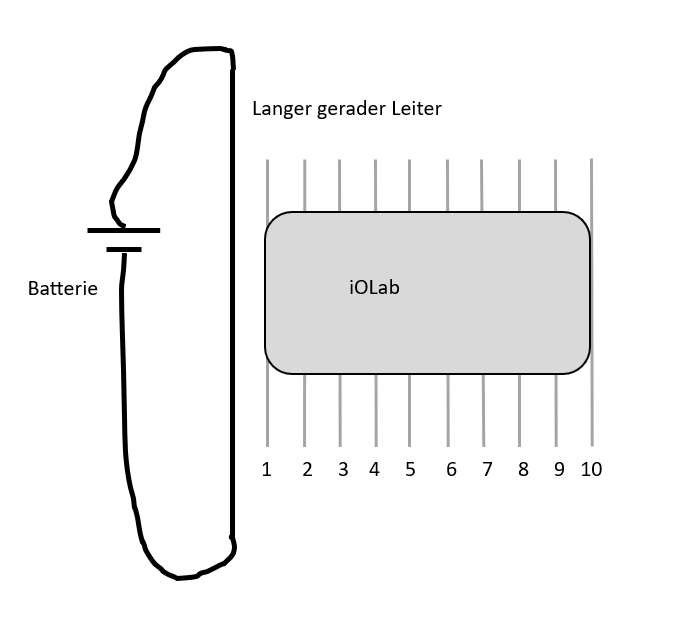
\includegraphics[width=7cm,keepaspectratio]{B2_Abbildung Aufbau2}
	\caption{Schematischer Aufbau des dritten Versuchs.}
	\label{fig:Ab2}
\end{figure} 
Für die erste Messung mit Magnetometer des IOLabs wird das Gerät direkt an das Kabel gelegt. Nun wird die Batterie für zwei Sekunden kurzgeschlossen. Dies wird nun für alle Abstände wiederholt. 